%Authors guidlines: http://royalsocietypublishing.org/instructions-authors
% 2500 words max (includes the title page, abstract, references, acknowledgements and figure/table legends)
% current version is around 3700. I think a big cut down can be done on the references.
% We allow a maximum of 4 displays, only 2 of which can be figures.

\documentclass[12pt,letterpaper]{article}
\usepackage{natbib}

%Packages
\usepackage{pdflscape}
\usepackage{fixltx2e}
\usepackage{textcomp}
\usepackage{fullpage}
%\usepackage{natbib}
\usepackage{float}
\usepackage{latexsym}
\usepackage{url}
\usepackage{epsfig}
\usepackage{graphicx}
\usepackage{amssymb}
\usepackage{amsmath}
\usepackage{bm}
\usepackage{array}
\usepackage[version=3]{mhchem}
\usepackage{ifthen}
\usepackage{caption}
\usepackage{hyperref}
\usepackage{amsthm}
\usepackage{amstext}
\usepackage{enumerate}
\usepackage[osf]{mathpazo}
\usepackage{dcolumn}
\usepackage{lineno}
\usepackage{longtable}
\pagenumbering{arabic}


%Pagination style and stuff % NC: Note that these are all syst biol specific.
\linespread{2}
\raggedright
\setlength{\parindent}{0.5in}
\setcounter{secnumdepth}{0} 
\renewcommand{\section}[1]{%
\bigskip
\begin{center}
\begin{Large}
\normalfont\scshape #1
\medskip
\end{Large}
\end{center}}
\renewcommand{\subsection}[1]{%
\bigskip
\begin{center}
\begin{large}
\normalfont\itshape #1
\end{large}
\end{center}}
\renewcommand{\subsubsection}[1]{%
\vspace{2ex}
\noindent
\textit{#1.}---}
\renewcommand{\tableofcontents}{}
%\bibpunct{(}{)}{;}{a}{}{,}

%---------------------------------------------
%
%       START
%
%---------------------------------------------

\begin{document}

%Running head
\begin{flushright}
Version dated: \today
\end{flushright}
\bigskip
\noindent RH: Morphological data availability in living mammals

\bigskip
\medskip
\begin{center}

\noindent{\Large \bf Morphological data availability in living mammals}
%Or: Missing cladistic data in living mammals - but I prefer the first one emphasizing on the availability of it. The data is not missing per se, it's just not coded!
% NC: sometimes the better title is one that answers the question rather than giving the topic. e.g., "Morphological data is lacking for living species" or similar

%Key words: Total Evidence method, data structure, phylogenetic, living, fossil, topology
\bigskip

\noindent {\normalsize \sc Thomas Guillerme$^1$$^,$$^2$$^,$$^*$ and Natalie Cooper$^1$$^,$$^2$$^,$$^3$}\\
\noindent {\small \it 
$^1$School of Natural Sciences, Trinity College Dublin, Dublin 2, Ireland.\\
$^2$Trinity Centre for Biodiversity Research, Trinity College Dublin, Dublin 2, Ireland.\\
$^3$Department of Life Sciences, Natural History Museum, Cromwell Road, London, SW7 5BD, UK.}\\
\end{center}
\medskip
\noindent{*\bf Corresponding author.} \textit{Zoology Building, Trinity College Dublin, Dublin 2, Ireland; E-mail: guillert@tcd.ie; Fax: +353 1 6778094; Tel: +353 1 896 2571.}\\ % NC: Might need to reconsider the email here as it won't be your email anymore when you leave. Or do you get to keep it forever? 
\vspace{1in}

%Line numbering
\modulolinenumbers[1]
\linenumbers

%---------------------------------------------
%
%       ABSTRACT
%
%---------------------------------------------
% NC: I've commented this out so I don't have to keep scrolling past in in the PDF
%\newpage
%\begin{abstract}
%Studying changes in global biodiversity through time and space is essential.
%For that we need methods to combine both palaeontological and neontological data.
%One promising method, the Total Evidence method, allows such thing but needs a lot of data.
%Especially cladistic data from living taxa to allow the fossil taxa to accurately branch in the trees.
%Despite two centuries of morphological studies on living taxa, scientists using and generating such data mainly focus on palaeontological data.
%Therefore, even in well known groups such as mammal, there is a huge gap in our knowledge of cladistic data for living mammals.
%In this study, using phylogenetic community structure methods, we quantify the availability of data in each mammalian order.
%And maybe at the end of the paper we propose some discussion on how to improve all that (go in museums!).
%\end{abstract}

%\noindent ()\\

%\vspace{1.5in}



%---------------------------------------------
%
%       INTRODUCTION
%
%---------------------------------------------

%NC: I've changed cladistic to morphological throughout but you might want to change it back...

\newpage 
\section{Introduction}
There is an increasing consensus among evolutionary biologists that studying both living and fossil taxa is essential for fully understanding macroevolutionary patterns and processes \citep{jacksonwhat2006,quentaldiversity2010,dietlconservation2011,slaterunifying2013,fritzdiversity2013,Wood01032013}.
For example, including both living and fossil taxa in evolutionary studies can improve the accuracy of timing diversification events \citep[e.g.][]{ronquista2012}, our understanding of relationships among lineages \citep[e.g.][]{beckancient2014}, and our ability to infer biogeographical patterns through time \citep[e.g.][]{Meseguer01032015}.
To perform such analyses it is necessary to combine living and fossil taxa in phylogenetic trees.
One increasingly popular method, the Total Evidence method \citep{eernissetaxonomic1993,ronquista2012}, combines molecular data from living taxa and morphological data from both living and fossil taxa in a supermatrix \citep[e.g.][]{pyrondivergence2011,ronquista2012,schragocombining2013,slaterunifying2013,beckancient2014,Meseguer01032015}, producing a phylogeny with living and fossil taxa at the tips. 
These phylogenies can be dated using methods such as tip-dating \citep{ronquista2012,Drummond01082012,Wood01032013,BEASTmaster} and incorporated into macroevolutionary studies (e.g. ).

A downside of the Total Evidence method is that it requires a lot of data.
One must collect molecular data for living taxa and morphological data for both living and fossil taxa; two types of data that require fairly different technical skills \citep[e.g.][]{meredithimpacts2011} \textit{vs.} \citep{O'Leary08022013}.
% NC: Is that really what these papers show? They use differnt data but they don't talk about the technical skills! Might be better just to say something like (e.g., PCR/sequencing vs. anatomical description)
Additionally, large chunks of this data can be difficult, or even impossible, to collect for every taxon present in the analysis.
For example, fossils very rarely have molecular data and incomplete fossil preservation may restrict the amount of morphological data available. % NC: Worth metioning fossil preservation here briefly as it is also an issue?
Additionally, since the molecular phylogenetics revolution, it has become less common to collect morphological characters for living taxa when molecular data is available \citep[e.g.][]{slaterphylogenetic2013,beckancient2014}.
%NC: Do these references actually say this??? Sounds like that's what you are saying
Unfortunately this missing data can lead to errors in phylogenetic inference; in fact, simulations show that the ability of the Total Evidence method to recover the correct phylogenetic topology decreases when there is a low overlap between morphological data in the living and fossil taxa \citep{GuillermeCooper}, regardless the overall amount of morphological data available for the fossils (or the amount of molecular data available for the living species).
The effect of missing data on topology is greatest when living taxa have little morphological data.
This is because (1) a fossil cannot branch in the correct clade if there is no overlapping morphological data in the clade; and (2) a fossil has a higher probability of branching within a clade with more morphological data available for living taxa, regardless of whether this is the correct clade or not \citep{GuillermeCooper}. 
This can lead to serious topological errors (see Figure ~\ref{Figure_missing_data_problem}). 

% NC: OK so I know we did a paper on this but you can't just cite it every sentence. Need to put in a few more refs to other people's work or just cite us once or twice. I've condensed it which should help

\begin{figure}[!htbp]
\centering
    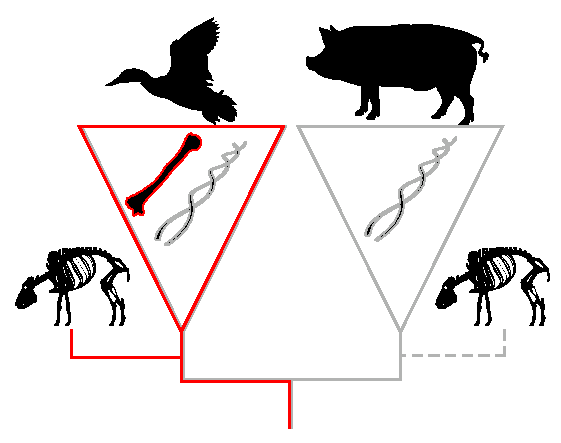
\includegraphics[width=1\textwidth]{MissingDataFigure.pdf}
\caption{Example of topological errors due to missing morphological data in living taxa.
The phylogeny contains two clades, Aves and Mammalia, with molecular data (grey) for both but only morphological data (red) for Aves.
If a mammalian fossil species (with no molecular data) is added to the phylogeny, it will erroneously branch with the Aves instead of the Mammalia because no morphological data will overlap between the fossil mammals and the living ones.}
\label{Figure_missing_data_problem}
\end{figure}

%What we're doing

The issues above highlight that it is crucial to have sufficient morphological data for living taxa in a clade before using a Total Evidence approach.
However, it is unclear how much morphological data for living taxa is actually available (i.e. already coded from specimens of living species and deposited in phylogenetic matrices), and how this data is distributed.
Intuitively, most people assume this kind of data has already been collected, but our experiences suggest otherwise.
To investigate this further, here we assess the amount of available morphological data for living mammals to determine whether sufficient data exists to build reliable Total Evidence phylogenies in this group.
We collected cladistic data from @256 phylogenetic matrices available online and measured the proportion of cladistic data available for each mammalian order.
Additionally, if the available data is randomly distributed across clades, the topological errors should be less extreme than if the data is biased towards particulars groups.
Therefore, in the mammalian orders where data was missing, we determined whether the available cladistic data was phylogenetically overdispersed or clustered. 
We find???
% NC: Needs some summing up sentence or a we find sentence?


%---------------------------------------------
%
%       METHODS
%
%---------------------------------------------
 
%\newpage

\section{Material and Methods}
\subsection{Matrices search}
To investigate the living mammals with available cladistic data, we downloaded cladistic matrices from three major public databases: morphobank (\texttt{http://www.morphobank.org/}) \citep{morphobank}, Graeme Lloyd's website (\texttt{http://graemetlloyd.com/}) and Ross Mounce's GitHub repository (\texttt{https://github.com/rossmounce}).
We downloaded all the matrices containing any living or/and fossil mammal taxa from these databases.
Additionally we ran a thorough Google Scholar search for matrices that might not have been uploaded on the previously mentioned data bases.
We downloaded the additional cladistic matrices from the 20 first Google search results matching with our selected keywords and with any of the 35 taxonomic levels (mammals Orders, Infraclasses and Class; see supplementary materials for detailed description of the procedure).
In total, we downloaded 256 % @@@ Number of matrices
matrices with 9411 % @@@ Number of living OTUs
operational taxonomic units (OTUs) from the combination of both searches (public repositories and Google Scholar). % link

%We transformed all the matrices to be in nexus format.
We standardised the taxonomic nomenclature by fixing invalid binomial inputs to match with the official taxonomic nomenclature rules (i.e. \textit{H. sapiens} was transformed in \textit{Homo sapiens}).
We assigned each species as being either living or fossil using a taxonomic matching algorithm described as follow: (1) we designated as living OTU all the OTUs that where either present in \citep{FritzTree} or \citep{wilson2005mammal}; (2) we designated as fossil OTUs all the OTUs that where present in the Paleobiology database and (3) for the OTUs neither labelled as living or fossil we tried to decompose the OTUs name (i.e. \textit{Homo$\_$sapiens} became \textit{Homo} and \textit{sapiens}) and tried to match the first element with any taxonomic level (Family, Genus, Species, etc.) from \citep{wilson2005mammal}. % link
The matching OTUs where labelled as living and the ones still not matching where ignored and labelled as non-applicable (NA; see supplementary material for more details on the taxonomic matching algorithm).

\subsection{Data availability analysis}
\subsubsection{Number of characters threshold}
From all the 256 % @@@ Number of matrices
matrices, we selected only the ones that coded at least 100 cladistic characters per OTU.
This arbitrary threshold of a minimal number of cladistic characters was chosen to be in adequacy with \citep{GuillermeCooper} and \citep{harrisonamong-character2014}.
Also this threshold avoids biases towards small matrices that could be either non-informative \citep{wagner2000} (e.g. too few characters not allowing character overlap among matrices) or that contained non-applicable characters \citep{Brazeau2011} (e.g. antlers ramification which is a only applicable to cervidae).

\subsubsection{Data availability}
To assess the data availability per mammal order, we calculated the percentage of OTUs with cladistic data for three different taxonomic levels: Family, Genus and Species.
We highlighted all the orders containing less than 25\% of living taxa with cladistic data because their amount of missing data ($>$75\%) was higher than in \citep{GuillermeCooper} and therefore likely to induce topological errors.
On the opposite, orders with up to 25\% of missing data (75\% of available data) were shown to have no significant effect on topology \citep{GuillermeCooper}.
We therefore used this value as a threshold of ``bad'' ($<$ 25\% available) and ``good'' ($>$ 75\% available) data coverage.

\subsubsection{Available data structure}
For the orders that contained OTUs with no cladistic data at any of the three different taxonomic levels (Family, Genus and Species), we investigated whether the structure of the available data was either (i) randomly distributed, (ii) over-dispersed or (iii) clustered by using cNet Relatedness Index (NRI) metric \citep{webb2002phylogenies} using the \texttt{picante} R package \citep{picante}.
The NRI quantifies the overall distribution of the observed data compared to a model where all the data is sampled for each OTU. Negative NRI values are showing more over-dispersed than expected by the null model (random) and positive values are showing more clustered data \citep{webb2002phylogenies}.
We choose NRI metric because is has been shown to be slightly less sensitive to the structure of the phylogeny (i.e. branch length and topology) \citep{NRI,journal.pone.0004390} but we also calculated two other common phylogenetic structure indices: Faith's Phylogenetic Distance (PD) \citep{Faith19921} and the Nearest Taxon Index (NTI) \citep{webb2002phylogenies}.
Both metrics are available in the Supplementary results.

%\subsubsection{Data improvement strategy}
%Too long for this paper and actually still a lot of work to do (transform the code of phylotargeting + come up with a valid strategy)

%---------------------------------------------
%
%       RESULTS
%
%---------------------------------------------

\section{Results}

\subsection{Data availability}
We extracted 1422 living mammal OTUs from the 256 matrices with a minimum of 6 and a maximum of 4541 coded cladistic characters per OTU.
After removing all the matrices with less than 100 cladistic characters, the number of extracted living mammals OTUs was down to 815.
11/28 orders have less than 25\% of OTUs with cladistic data at a species level and 24/28 orders have less than 75\% taxa with available cladistic data.
At the Genus level however only 3/28 orders have less than 25\% of taxa with cladistic data and 16/28 have less than 75\%.
Finally, at the family level no order has less than 25\% taxa with available cladistic data and only 5/28 have less than 75\% (table \ref{Table_morpho_taxa_proportion}).

\renewcommand\baselinestretch{1.2}\selectfont
\begin{center}
% latex table generated in R 3.1.1 by xtable 1.7-3 package
% Mon Feb 23 12:34:36 2015
\begin{longtable}{llll}
  \hline
Order & Taxonomic level & Fraction of OTUs & Percentage of OTUs \\ 
  \hline
Monotremata & Family & 2/2 & 100 \\ 
  Monotremata & Genus & 2/3 & 66.67 \\ 
  Monotremata & Species & 2/4 & 50 \\ 
  Didelphimorphia & Family & 1/1 & 100 \\ 
  Didelphimorphia & Genus & 16/16 & 100 \\ 
  Didelphimorphia & Species & 40/84 & 47.62 \\ 
  Paucituberculata & Family & 1/1 & 100 \\ 
  Paucituberculata & Genus & 2/3 & 66.67 \\ 
  Paucituberculata & Species & 2/5 & 40 \\ 
  Microbiotheria & Family & 1/1 & 100 \\ 
  Microbiotheria & Genus & 1/1 & 100 \\ 
  Microbiotheria & Species & 1/1 & 100 \\ 
  Notoryctemorphia & Family & 1/1 & 100 \\ 
  Notoryctemorphia & Genus & 1/1 & 100 \\ 
  \textbf{Notoryctemorphia} & \textbf{Species} & \textbf{0/2} & \textbf{0} \\ 
  Dasyuromorphia & Family & 2/2 & 100 \\ 
  Dasyuromorphia & Genus & 7/22 & 31.82 \\ 
  \textbf{Dasyuromorphia} & \textbf{Species} & \textbf{8/64} & \textbf{12.5} \\ 
  Peramelemorphia & Family & 2/2 & 100 \\ 
  Peramelemorphia & Genus & 7/7 & 100 \\ 
  Peramelemorphia & Species & 16/18 & 88.89 \\ 
  Diprotodontia & Family & 9/11 & 81.82 \\ 
  Diprotodontia & Genus & 20/38 & 52.63 \\ 
  \textbf{Diprotodontia} & \textbf{Species} & \textbf{16/126} & \textbf{12.7} \\ 
  Afrosoricida & Family & 2/2 & 100 \\ 
  Afrosoricida & Genus & 17/17 & 100 \\ 
  Afrosoricida & Species & 23/42 & 54.76 \\ 
  Macroscelidea & Family & 1/1 & 100 \\ 
  Macroscelidea & Genus & 4/4 & 100 \\ 
  Macroscelidea & Species & 5/15 & 33.33 \\ 
  Tubulidentata & Family & 1/1 & 100 \\ 
  Tubulidentata & Genus & 1/1 & 100 \\ 
  Tubulidentata & Species & 1/1 & 100 \\ 
  Hyracoidea & Family & 1/1 & 100 \\ 
  Hyracoidea & Genus & 1/3 & 33.33 \\ 
  Hyracoidea & Species & 1/4 & 25 \\ 
  Proboscidea & Family & 1/1 & 100 \\ 
  Proboscidea & Genus & 1/2 & 50 \\ 
  Proboscidea & Species & 1/3 & 33.33 \\ 
  Sirenia & Family & 2/2 & 100 \\ 
  Sirenia & Genus & 2/2 & 100 \\ 
  Sirenia & Species & 2/4 & 50 \\ 
  Cingulata & Family & 1/1 & 100 \\ 
  Cingulata & Genus & 8/9 & 88.89 \\ 
  \textbf{Cingulata} & \textbf{Species} & \textbf{6/25} & \textbf{24} \\ 
  Pilosa & Family & 3/5 & 60 \\ 
  Pilosa & Genus & 3/5 & 60 \\ 
  \textbf{Pilosa} & \textbf{Species} & \textbf{3/29} & \textbf{10.35} \\ 
  Scandentia & Family & 2/2 & 100 \\ 
  Scandentia & Genus & 2/5 & 40 \\ 
  \textbf{Scandentia} & \textbf{Species} & \textbf{2/20} & \textbf{10} \\ 
  Dermoptera & Family & 1/1 & 100 \\ 
  Dermoptera & Genus & 1/2 & 50 \\ 
  Dermoptera & Species & 1/2 & 50 \\ 
  Primates & Family & 15/15 & 100 \\ 
  Primates & Genus & 48/68 & 70.59 \\ 
  \textbf{Primates} & \textbf{Species} & \textbf{56/351} & \textbf{15.95} \\ 
  Rodentia & Family & 10/32 & 31.25 \\ 
  \textbf{Rodentia} & \textbf{Genus} & \textbf{20/451} & \textbf{4.43} \\ 
  \textbf{Rodentia} & \textbf{Species} & \textbf{10/2095} & \textbf{0.48} \\ 
  Lagomorpha & Family & 1/2 & 50 \\ 
  \textbf{Lagomorpha} & \textbf{Genus} & \textbf{1/12} & \textbf{8.33} \\ 
  \textbf{Lagomorpha} & \textbf{Species} & \textbf{1/86} & \textbf{1.16} \\ 
  Erinaceomorpha & Family & 1/1 & 100 \\ 
  Erinaceomorpha & Genus & 10/10 & 100 \\ 
  Erinaceomorpha & Species & 21/22 & 95.45 \\ 
  Soricomorpha & Family & 3/4 & 75 \\ 
  Soricomorpha & Genus & 19/43 & 44.19 \\ 
  \textbf{Soricomorpha} & \textbf{Species} & \textbf{19/392} & \textbf{4.85} \\ 
  Chiroptera & Family & 13/18 & 72.22 \\ 
  Chiroptera & Genus & 68/202 & 33.66 \\ 
  \textbf{Chiroptera} & \textbf{Species} & \textbf{108/1054} & \textbf{10.25} \\ 
  Pholidota & Family & 1/1 & 100 \\ 
  Pholidota & Genus & 1/1 & 100 \\ 
  Pholidota & Species & 3/8 & 37.5 \\ 
  Carnivora & Family & 11/15 & 73.33 \\ 
  \textbf{Carnivora} & \textbf{Genus} & \textbf{30/125} & \textbf{24} \\ 
  \textbf{Carnivora} & \textbf{Species} & \textbf{42/283} & \textbf{14.84} \\ 
  Perissodactyla & Family & 3/3 & 100 \\ 
  Perissodactyla & Genus & 6/6 & 100 \\ 
  Perissodactyla & Species & 7/16 & 43.75 \\ 
  Cetartiodactyla & Family & 20/21 & 95.24 \\ 
  Cetartiodactyla & Genus & 76/128 & 59.38 \\ 
  Cetartiodactyla & Species & 106/311 & 34.08 \\ 
   \hline
\hline
\end{longtable}

\end{center}
\renewcommand\baselinestretch{2}\selectfont

\subsection{Available data structure}
Among the orders containing OTUs with no available cladistic data, only two orders are significantly clustered: Carnivora and Chiroptera both at the species and the genus level (table~\ref{Table_data_structure}).

\renewcommand\baselinestretch{1.2}\selectfont
\begin{center}
% latex table generated in R 3.1.1 by xtable 1.7-3 package
% Fri Feb 27 10:08:44 2015
\begin{longtable}{lllll}
\caption{Data structure for the orders with OTUs without morphological data per taxonomic level. When the Net Relatedness Index (NRI) is negative, the OTUs are more dispersed than expected by chance (random); when the NRI is positive, the OTUs are more clustered by expected by chance. The p-value indicates the significance in difference from the null model (random).} \\ 
  \hline
Order & Taxonomic level & Percentage of OTUs & NRI & p-value \\ 
  \hline
Monotremata & Genus & 66.667 & -0.695 & 0.663 \\ 
  Monotremata & Species & 50 & -0.966 & 0.566 \\ 
  Didelphimorphia & Species & 47.619 & -1.33 & 0.915 \\ 
  Paucituberculata & Genus & 66.667 & -0.756 & 0.682 \\ 
  Paucituberculata & Species & 40 & -0.64 & 0.493 \\ 
  Dasyuromorphia & Genus & 31.818 & -1.102 & 0.894 \\ 
  Dasyuromorphia & Species & 12.5 & -1.098 & 0.93 \\ 
  Peramelemorphia & Species & 88.889 & -0.55 & 0.748 \\ 
  Diprotodontia & Family & 81.818 & -0.349 & 0.551 \\ 
  Diprotodontia & Genus & 52.632 & -0.31 & 0.595 \\ 
  Diprotodontia & Species & 12.698 & -0.975 & 0.849 \\ 
  Afrosoricida & Species & 54.762 & 1.555 & 0.077 \\ 
  Macroscelidea & Species & 33.333 & -0.474 & 0.66 \\ 
  Sirenia & Species & 50 & -0.957 & 0.845 \\ 
  Cingulata & Genus & 88.889 & 1.31 & 0.229 \\ 
  Cingulata & Species & 24 & 0.648 & 0.223 \\ 
  Pilosa & Family & 60 & -0.603 & 0.891 \\ 
  Pilosa & Genus & 60 & -0.877 & 0.795 \\ 
  Pilosa & Species & 10.345 & -1.508 & 0.997 \\ 
  Scandentia & Genus & 40 & -0.747 & 0.639 \\ 
  Scandentia & Species & 10 & -1.259 & 0.984 \\ 
  Primates & Genus & 70.588 & -0.302 & 0.607 \\ 
  Primates & Species & 15.954 & -1.504 & 0.951 \\ 
  Rodentia & Family & 31.25 & 0.113 & 0.395 \\ 
  Rodentia & Genus & 4.435 & -1.032 & 0.848 \\ 
  Rodentia & Species & 0.477 & -0.967 & 0.856 \\ 
  Erinaceomorpha & Species & 95.455 & -0.777 & 0.914 \\ 
  Soricomorpha & Family & 75 & -0.95 & 0.619 \\ 
  Soricomorpha & Genus & 44.186 & 1.157 & 0.116 \\ 
  Soricomorpha & Species & 4.847 & -1.869 & 0.977 \\ 
  Chiroptera & Family & 72.222 & 0.866 & 0.201 \\ 
  \textbf{Chiroptera} & \textbf{Genus} & \textbf{33.663} & \textbf{18.87} & \textbf{0.001} \\ 
  \textbf{Chiroptera} & \textbf{Species} & \textbf{10.247} & \textbf{20.112} & \textbf{0.001} \\ 
  Pholidota & Species & 37.5 & 1.14 & 0.175 \\ 
  Carnivora & Family & 73.333 & 0.517 & 0.285 \\ 
  \textbf{Carnivora} & \textbf{Genus} & \textbf{24} & \textbf{4.014} & \textbf{0.002} \\ 
  \textbf{Carnivora} & \textbf{Species} & \textbf{14.841} & \textbf{17.954} & \textbf{0.001} \\ 
  Perissodactyla & Species & 43.75 & 0.733 & 0.199 \\ 
  Cetartiodactyla & Family & 95.238 & 0.352 & 0.193 \\ 
  Cetartiodactyla & Genus & 59.375 & -3.221 & 1 \\ 
  Cetartiodactyla & Species & 34.084 & -2.768 & 1 \\ 
   \hline
\hline
\label{Table_data_structure}
\end{longtable}

\end{center}
\renewcommand\baselinestretch{2}\selectfont

Two contrasted results are shown on figure \ref{Figure_example_coverage} with randomly distributed data in Cetartiodactyla (figure \ref{Figure_example_coverage}-A) and clustered available data in Carnivora (mainly Canidae; figure \ref{Figure_example_coverage}-B).

\begin{figure}[!htbp]
\centering
    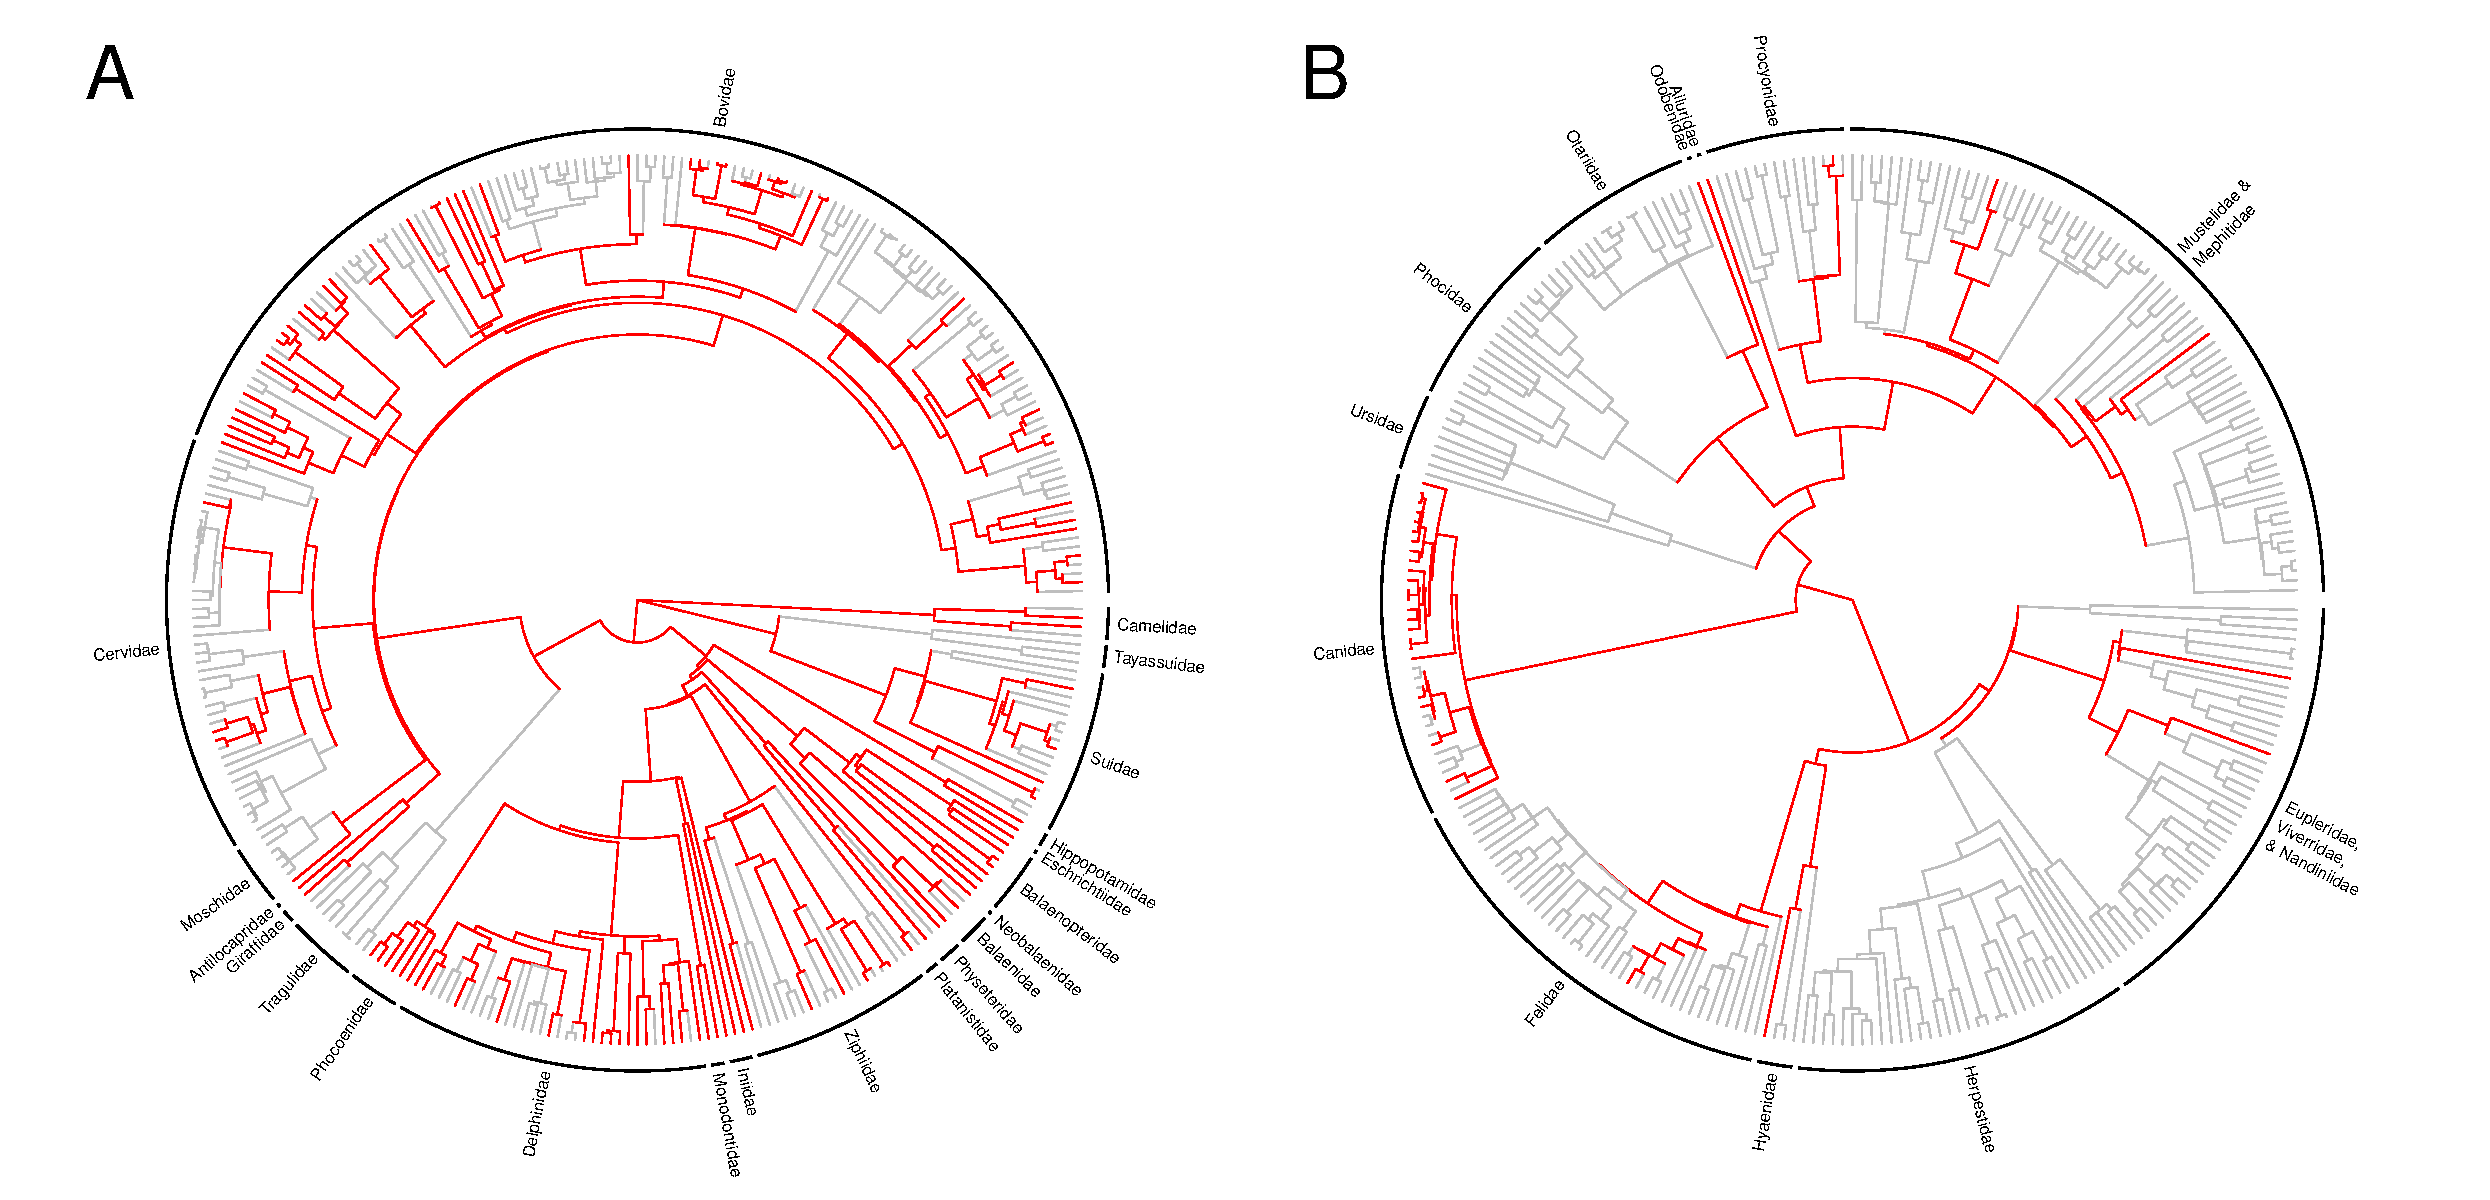
\includegraphics[width=1\textwidth]{example_coverage.pdf}
\caption{Distribution of available cladistic data across two different clades (A: Cetartiodactyla; B: Carnivora).
Edges are colored in grey when no cladistic data is available or in red when data is available.}
\label{Figure_example_coverage}
\end{figure}


%\subsection{Data improvement strategy}


%---------------------------------------------
%
%       DISCUSSION
%
%---------------------------------------------

\section{Discussion}
Our results show that even though relations among living mammals are well known in a molecular framework \citep[e.g.][]{FritzTree,meredithimpacts2011,May-Collado-PeerJ} only little cladistic data is available.
This is primarily due to the fact that that cladistic studies are mainly focusing on fossil taxa rather than living taxa \citep[e.g.][]{O'Leary08022013,ni2013oldest}.
However, data availability varies in its structure as well as across taxonomic levels.
Higher taxonomic levels are always better sampled than lower ones (table \ref{Table_morpho_taxa_proportion}) and within these taxonomic levels, the structure of available data is mostly random apart for two orders (table \ref{Table_data_structure})b.

%\subsection{Data availability}
The amount of living taxa with no available cladistic data was surprisingly high at the species level: 24/28 orders have less than 75\% taxa with available cladistic data (and two of the 28 orders are monospecific!).
This threshold of 75\% available data is the maximum amount of possible missing data (25\%) before having a significant effect on the topology of Total Evidence trees \citep{GuillermeCooper}.
Beyond this threshold, there is a noteworthy displacement of the wildcard taxa (\textit{sensu} \citep{kearneyfragmentary2002}) as well as a important decrease in the conservation of clades \citep{GuillermeCooper}.
At the species level within most orders of mammals, it is therefore likely to see topological artefacts for the placement of fossil taxa.
However, the data availability seems to be less an issue at higher taxonomic level (i.e. the Genus and the Family level).
This point is important to consider from a practical point of view because of the slight discrepancy between the neontological and the palaeontological concept of species.
While neontological species are described on accurately measured morphology, genetic distance, spacial distribution and even behaviour \citep[e.g.][]{kellymolecular2014}, palaeontological data can be based only on morphological, spatial and temporal data \citep[e.g.][]{ni2013oldest}.
Because of this difference between neontological species (\textit{sensu} reproductive isolates) and paleontological species (\textit{sensu} morpho-species %or "morphological clusters"?
), most palaeontological studies are using the Genus level for their smallest OTU \citep[e.g.][]{ni2013oldest,O'Leary08022013}.
In this frame of palaeontological data usage, the data availability at the Genus level in living mammals should be our priority concern.

%\subsection{Available data structure}
Regardless the low level of available data, it is encouraging that for most orders (except Carnivora and Chiroptera), data is randomly distributed across the phylogeny.
%Therefore, it is likely that the addition of fossil taxa within these orders will not be biased by oversampling but will probably branch near the taxa that has the most similar available data (as expected).
There are three different scenarii, regarding the distribution of the available data, for predicting how fossils can branch in relation to living taxa.
When only few data is available, the ideal scenario will be that it is over-dispersed (i.e. that there is data in at least every sub-clade) in order to maximize the possibilities of the fossil to branch in the right clade.
In the second scenario, when the data is randomly distributed we expected no special bias in the placement of the fossil \citep{GuillermeCooper}.
However, in the third scenario, when the data is clustered we expect two major biases to occur: (1) first, the fossil will not be able to branch within a clade containing no data (e.g. Herpestidae in Carnivora; figure \ref{Figure_missing_data_problem} and \ref{Figure_example_coverage}-B), and (2) second, the fossil will have a higher probability, at random, to branch within the clade containing most of the available data (e.g. a Carnivora fossil will have more chance to branch, randomly, to the Canidae clade than any other clade in Carnivora; figure \ref{Figure_example_coverage}-B).
This means that fossils with uncertain phylogentic affinities (\textit{Incertae sedis}) will have a higher probability of branching by chance within the most sampled clade.

%For example in Carnivora, their is no available data for Herpestidae, therefore any fossil Herpestidae will not be able to be correctly placed in the phylogeny (figure ~\ref{Figure_example_coverage}-B.
%On the other hand, any Carnivora fossil with uncertain phylogenetic affinities (\textit{Incertae sedis} will have a higher probability of branching by chance within the Canidae because they are oversampled within the Carnivora (figure ~\ref{Figure_example_coverage}-B.

%Caveats
In this study, we treated all cladistic matrices to be equal in a similar way that molecular matrices are: for example if a matrix A contains 100 characters for taxa X and Y, and a matrix B contains 50 characters for taxa X and Z, we assumed that both matrices can be combined in a supermatrix containing 150 characters for taxon X, 100 for taxon Y and 50 for taxon Z.
However, it is clear that cladistic data cannot be treated that way \citep{Brazeau2011}.
In fact, for the same taxon, some characters might overlap (e.g. matrix A has a character coding for the shape of a particular morphological feature and matrix B as a first character coding for the presence of this morphological feature and a second one coding for its shape; in this case, these three characters are compound characters \citep{Brazeau2011}).
However, in reasonably sized matrices ($>$ 100 characters \citep{GuillermeCooper,harrisonamong-character2014} it is more likely that a number of characters are consistently conserved among the different matrices (e.g. within primates literature, the character \textit{p7} - the size of the $4^{th}$ lower premolar paraconid - is consistent for more than 15 years \citep{ross1998phylogenetic,seiffert2003fossil,marivaux2005anthropoid,seiffert2005basal,bloch2007new,kay2008anatomy,silcox2008biogeographic,seiffert2009convergent,tabuce2009anthropoid,boyer2010astragalar,seiffert2010fossil,marivaux2013djebelemur,ni2013oldest}).
A conservative approach to avoid compound characters could be to select only the most recent matrix for each group.

%Let's code some data
Following the recommendations in \citep{GuillermeCooper}, one should code cladistic characters for a maximum of living species in order to improve the topology of Total Evidence trees containing both living and fossil taxa.
Since the data for living mammals is usually easily available in world wide vast natural history collections, we propose that an increased effort in coding morphological characters from living species should be done via engaging in collaborative data collection projects through web portals such as \textit{morphobank} \citep{morphobank}.

%Biology letters various stuff
\section{Ethics statement}
\section{Data accessibility statement}
All data is available and reproducible on GitHub.
\section{Authors’ contributions statement}
Conceived and designed the experiments: TG NC. Performed the experiments: TG. Analyzed the data: TG. Wrote the paper: TG NC.
\section{Acknowledgements}
Nick Matzke, April Wright, David Bapst and Graeme Lloyd. %Or whatever order.
\section{Funding statement}
This work was funded by a European Commission CORDIS Seventh Framework Programme (FP7) Marie Curie CIG grant (proposal number: 321696).

\bibliographystyle{sysbio}
\bibliography{References}


%\section{SOM}
\newcommand{\beginsupplement}{%
    \setcounter{table}{0}
    \renewcommand{\thetable}{S\arabic{table}}%
    \setcounter{figure}{0}
    \renewcommand{\thefigure}{S\arabic{figure}}%
}
\beginsupplement

\noindent{\Large \bf Supplementary Material}

\bigskip

\section{Data collection}
1- Data collection: key words, clade (ordinal) metacharacters, Google Search terms, Google Search protocol, Google Search rarefaction curve.

\subsection{Public repositories}
We downloaded available matrices containing fossil and/or living mammal taxa from the three following data bases using the following list of keywords:

\texttt{Mammalia; Monotremata; Marsupialia; Placentalia; Macroscelidea; Afrosoricida; Tubulidentata; Hyracoidea; Proboscidea; Sirenia; Pilosa; Cingulata; Scandentia; Dermoptera; Primates; Lagomorpha; Rodentia; Erinaceomorpha; Soricomorpha; Cetacea; Artiodactyla; Cetartiodactyla; Chiroptera; Perissodactyla; Pholidota; Carnivora; Didelphimorphia; Paucituberculata; Microbiotheria; Dasyuromorphia; Peramelemorphia; Notoryctemorphia; Diprotodontia}.

Details about each public repository specific search option is listed below. Note that some matrices have been downloaded from more than one database but that it is not an issue since we are interested in the total number of living OTUs and that if some where present in more than one matrix, they still only counted as a unique OTU.

\subsubsection{Morphobank}
We accessed the Morphobank repository (\texttt{http://www.morphobank.org/}) on the 5th of December 2014 and used the keywords listed above in the search menue. We downloaded the data associated with each project matching with the keyword.

\subsubsection{Graeme Lloyd}
We accessed Graeme Lloyd's website repository (\texttt{http://graemetlloyd.com/}) on the 5th of December 2014 and downloaded all the matrices that were available with a direct download link in the mammal data section of the website (\texttt{http://graemetlloyd.com/matrmamm.html}).

\subsubsection{Ross Mounce}
We accessed Ross Mounce's GitHub repository (\texttt{https://github.com/rossmounce}) on the 2nd of December 2014 and downloaded every 601 matrix. We then ran a shell script to select only the matrices that had any text element that match with one of the search terms. To make the matrix selection more thorough, we ignored the keywords case as well as the latin suffix (\textit{ia}, \textit{ata}, \textit{ea}, and \textit{a}).

\subsection{Google scholars}
To make sure we didn't miss any extra matrix that wasn't available on one of these repository, we ran a Google Scholar search on the 5th of January. We used the following key words:

\texttt{\textit{order} ("morphology" OR "morphological" OR "cladistic") AND characters matrix paleontology phylogeny}

were \textit{order} was replaced by all the keywords listed above. For each 33 keywords, we selected the 20 first papers to match the Google search published since 2010 resulting in 660 papers. Among these papers, not all contained relevant data (discrete morphological characters AND mammalian data). We selected only the 20 first results per search term to avoid downloading articles that were to irrelevant. Among the 660 papers, only 50 contained a total of 425 extra living OTUs (figure ~\ref{Supp_figure_google_searches}).
Also we decided to select only the articles published since 2010 because nearly every one of the recent published matrix contains both a fraction of morphological characters and OTUs from previous studies. For example in primates the character \textit{p7} coded first by \cite{ross1998phylogenetic} is reused with the same living species in \cite{seiffert2003fossil}, \cite{marivaux2005anthropoid}, \cite{seiffert2005basal}, \cite{bloch2007new}, \cite{bloch2007new}, \cite{kay2008anatomy}, \cite{silcox2008biogeographic}, \cite{seiffert2009convergent}, \cite{tabuce2009anthropoid}, \cite{boyer2010astragalar}, \cite{seiffert2010fossil}, \cite{marivaux2013djebelemur} and \cite{ni2013oldest}.

\begin{figure}[!htbp]
\centering
    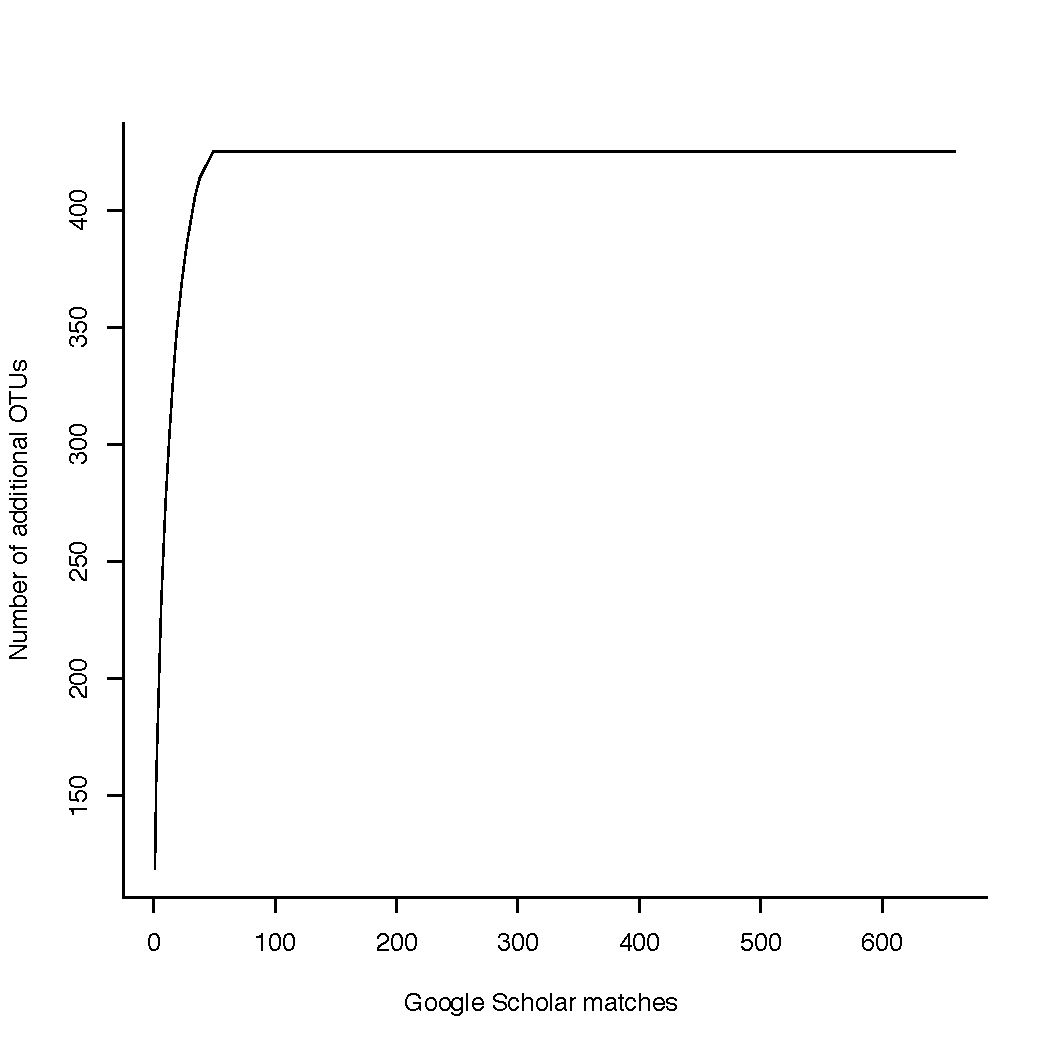
\includegraphics[width=1\textwidth]{Supplementary/Supp_figure_google_searches.pdf}
\caption{Google searches additional OTUs rarefaction curve. The x axis represent the number of google scholar matches (papers, books or abstracts) and the y axis represents the cumulative number of additional living OTUs per google scholar match.}
\label{Supp_figure_google_searches}
\end{figure}

\subsection{Standardising the matrices}
We transformed all the non-nexus matrices (tnt, word, excel, jpeg) to nexus format manually. We then cleaned the nexus matrices by removing any extra information (trees, continuous characters, morphological characters description, molecular data) to end up with nexus matrices containing only the discrete morphological data. We then manually fixed the wrong bionomial names format (e.g. \textit{H. sapiens}) into the correct ones (e.g. \textit{Homo sapiens}) using the abbreviation list in the concerned publications. 

\subsection{Selecting the living OTUs}
Finally we applied a taxonomic matching algorithm to classify the OTUs as either living or fossil. The algorithm is matching every OTU name from every matrix with one of the following taxonomic references: the list of taxa from the Fritz \textit{et al.} supertree (2009) \cite{FritzTree}; the taxonomic list from the Wilson and Reeder's Mammals Species of the World (2005) \cite{wilson2005mammal} and the list of all the mammal fossil from the Paleobio Database (\texttt{http://paleobiodb.org/cgi-bin/bridge.pl?a=login}) accessed on the 13th of Janurary 2015. The OTUs that matched with one of the two first references were considered as living OTUs, the OTUs matching with the third reference were considered as fossil OTUs, finally, the OTUs matching with non of the references were discarded (figure ~\ref{Supp_figure_Taxonomic_algorithm}).

\begin{figure}[!htbp]
\centering
    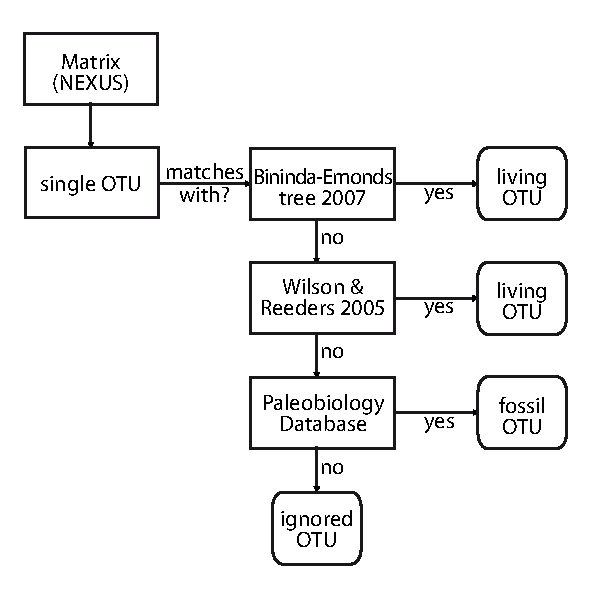
\includegraphics[width=1\textwidth]{Supplementary/Supp_figure_Taxonomic_algorithm.pdf}
\caption{Taxonomic matching algorithm used in this study. For each matrix, each operational taxonomic units (OTU) is matched with the super tree from Fritz 2009. If the OTU matches, then it is classified as living. Else it is matched with the Wilson \& Reeders 2005 taxonomy list. If the OTU matches, then it is classified as living. Else it is matched with the Paleo Database list of mammals. If the OTU matches, then it is classified as fossil. Else it is ignored.}
\label{Supp_figure_Taxonomic_algorithm}
\end{figure}

\bibliographystyle{vancouver}
\bibliography{Supp_References}


\section{Data structure}
%Tables
%Figures

\section{Supplementary results}



%END
\end{document}
